\documentclass[11pt,a4paper]{moderncv}
%\usepackage{amsmath}
%\usepackage{amssymb}
\usepackage{calc}
%\usepackage{caption}
\usepackage{color}
%\usepackage{commath}
%\usepackage{enumitem}
\usepackage{fancyhdr}
%\usepackage{float}
\usepackage{graphicx}
%\usepackage{hyperref}
\usepackage{lastpage}
%\usepackage{listings}
%\usepackage{mathtools}
\usepackage{pdfpages}
%\usepackage{siunitx}
%\usepackage{tikz}
\usepackage{biblatex}
\usepackage{todonotes}

\moderncvtheme[blue]{classic}
\usepackage[utf8]{inputenc}
\usepackage[scale=0.8]{geometry}
\recomputelengths

\addbibresource{references.bib}

\newcommand{\sep}{$~\bullet~$}
\newcommand{\osscontrib}[3]{\item[#1] #2\hfill\\See #3.}

\firstname{Taran}
\familyname{Lynn}
\title{Linux Engineer}
%\address{12 somestreet}{3456 somecity}
\mobile{(707) 372-3259}
\email{taranlynn0@gmail.com}

\extrainfo{\\
  Personal Site: \url{http://lambda-11235.github.io/}\\
  GitHub: \url{https://github.com/lambda-11235/}\\
  LinkedIn: \url{https://www.linkedin.com/in/taran-lynn/}
}

%\quote{Test}


\begin{document}
\maketitle

\section*{Education}

\begin{itemize}
\item 2019 BS in Computer Science and Engineering from U.C. Davis
  (GPA 3.98).

\item 2022 MS in Computer Science from U.C. Davis (GPA 3.85).
\end{itemize}


\section*{Specialty}

I specialize in computer network infrastructure.
My previous work has focused on researching TCP congestion control
algorithms and AQM, with a focus on reducing end-to-end tail latency.
Now my focus has shifted to applying these methods to cloud based networks.
I have also briefly worked on optimizing HPC systems with deep learning.


\section*{Skills}

\begin{description}
    \item[Programming Languages]
      C
      \sep C++
      \sep Python
      \sep Haskell
      \sep Scala
      \sep Java
        %\fbox{Lua}
        %\fbox{Rust}
        %\fbox{Coq}
        %\fbox{Prolog}
        %\fbox{Erlang}
        %\fbox{Clojure}
        %\fbox{Go}

    \item[Experience With]
      Networking
      \sep TCP Congestion Control
      \sep AQM
      \sep AWS (IoT \& Lambda)
      \sep OpenStack
      \sep Control Systems
      \sep Deep Learning
      \sep Tensorflow
      \sep PyTorch
      \sep Docker
      \sep HPC
      \sep Slurm
      % \fbox{Software Transactional Memory (STM);
      % \fbox{Functional Reactive Programming (FRP);
\end{description}


\section*{Papers}

\begin{itemize}
\item \fullcite{Lynn2020}

\item \fullcite{TCPD}
\end{itemize}

\section*{Presentations}

\begin{description}
    \item[Impact of Buffer Size on a Congestion Control Algorithm Based on Model Predictive Control]
        \hfill\\
        Presented at the 2019 Workshop on Buffer Sizing at Stanford, Ca.\\
        \url{http://buffer-workshop.stanford.edu/papers/paper14.pdf}\\
        \url{http://buffer-workshop.stanford.edu/slides/mpc.pdf}
\end{description}


\section*{University Projects}

\begin{description}
    \item[Model Predictive Congestion Control] \hfill
        %This is a research project whose aim is to develop a new TCP congestion
        %control algorithm that provides a smooth signal across dedicated WANs.
        %To do this the algorithm employs concepts from model predictive control
        %theory.
        %The algorithm also allows users to dynamically set pacing rates on a per
        %flow basis.
        %Implementations have been developed for both the TCP congestion control
        %and qDisc layers in the Linux kernel.

        \begin{itemize}
        \item New TCP congestion control algorithm providing a smooth
          RTT signal across dedicated WANs.

        \item Based on concepts from model predictive control.

        \item Implementations developed for both the TCP congestion
          control and qDisc layers in the Linux kernel.
        \end{itemize}

    \item[Randomizing Malloc for Security] \hfill
        %This project aimed to disrupt certain classes of buffer overflow attacks
        %that target malloc metadata.
        %Such attacks require malloc to allocate memory chunks in a contiguous,
        %predictable order.
        %To counteract this we randomized the spacing between the chunks, which
        %also had the effect of randomizing allocation order in some cases.
        %We submitted a paper detailing the modification to the Hawaii
        %International Conference on System Sciences (HICSS) in Spring of 2019.

        \begin{itemize}
        \item Expanded on method to disrupt certain classes of buffer
          overflow attacks that target malloc metadata.

        \item Main contribution was randomizing spacing between
          malloc's allocated memory chunks.
        \end{itemize}

      \item[Optimizing HPC Scheduling with LSTM Networks] \hfill
        %As part of a graduate course on deep learning I worked on a
        %team project with the goal of optimizing scheduling algorithms in
        %high-performance computing (HPC) centers.
        %This project was done in partnership with UC Davis' HPC Core
        %Facilities (HPCCF).
        %The eventual outcome was the development of a long-short term
        %memory (LSTM) network to predict job runtimes and memory usage.
        %I am continuing this work beyond the graduate course, in order to
        %extend the LSTM network into a recommendation system.

        \begin{itemize}
        \item Part of a graduate course on deep learning.
            
        \item Done in partnership with UC Davis' HPC Core Facilities
          (HPCCF).

        \item Used long-short term memory (LSTM) network to predict
          HPC job runtimes and memory usage, with the eventual goal of
          optimizing scheduling algorithms in high-performance
          computing (HPC) centers.
        \end{itemize}
\end{description}


\section*{Open Source Contributions}

\begin{description}
    \osscontrib{Idris}{I wrote documentation on the codata keyword.}{\url{https://github.com/idris-lang/Idris-dev/pull/3094/}}

    \osscontrib{NixOS}{I maintain several packages in their repository.}{\url{https://github.com/NixOS/nixpkgs/}}

    \osscontrib{The Secret Chronicles of Dr. M}{I helped port the game
    from SDL to SFML.}{\url{https://secretchronicles.org/en/}}

    \osscontrib{Red Eclipse}{I contributed custom content to their community
    repository.}{\url{https://www.redeclipse.net/}}
\end{description}

\subsection*{Personal Open Source Repositories}

\begin{description}
    \item[TTyped] A dependently typed language directly based off of
        Coquand's Calculus of Constructions.

    \item[debtTools] A command line python program to help users track
        and calculate payments for compound interest debt.
%        Also includes a paper that derives key formulas from first
%        assumptions.
%
    \item[Markov's Password] A random password generator based off of
        the XKCD comic ``Password Strength''
        (\url{https://www.xkcd.com/936/}).
%        It uses a variation of Markov chains to generate a sequence of
%        random, made up, and pronounceable words.
%        A version that uses a Hidden Markov Model is also being worked
%        on.
%
    \item[FarRP] A library for functional reactive programming that
        leverages dependent types in the Idris.
%        It is based on Neil Sculthorpe and Henrik Nilsson's paper "Safe
%        Functional Reactive Programming through Dependent Types."
\end{description}


\section*{Awards}

\begin{itemize}
    \item Received 2019 U.C. Davis Computer Science Departmental Citation.
\end{itemize}

\section*{Fellowships and Grants}

\begin{itemize}
\item Received the Towards Outstanding Postgraduate Students (TOPS) Award.
  This is an internal award provided by the College of Engineering at UC Davis.
\end{itemize}
%
%
%\section*{Notable Courses Taken}
%
%%\newcommand{\course}[2]{\fbox{#1 (#2)}}
%\newcommand{\course}[2]{#1}
%
%    \course{Algorithm Design}{ECS 122A/B}
%\sep\course{Circuits I/II}{ENG 17/EEC 100}
%\sep\course{Computer Architecture}{ECS 154A/B}
%\sep\course{Embedded Systems}{EEC 172}
%\sep\course{Machine Learning}{ECS 171}
%\sep\course{Operating Systems}{ECS 150}
%\sep\course{Parallel Architectures}{ECS 158}
%\sep\course{Deep Learning}{ECS 289G}
%
%\section*{References}
%
%References can be provided upon request.
%
%%\section*{Unofficial Transcript}
%%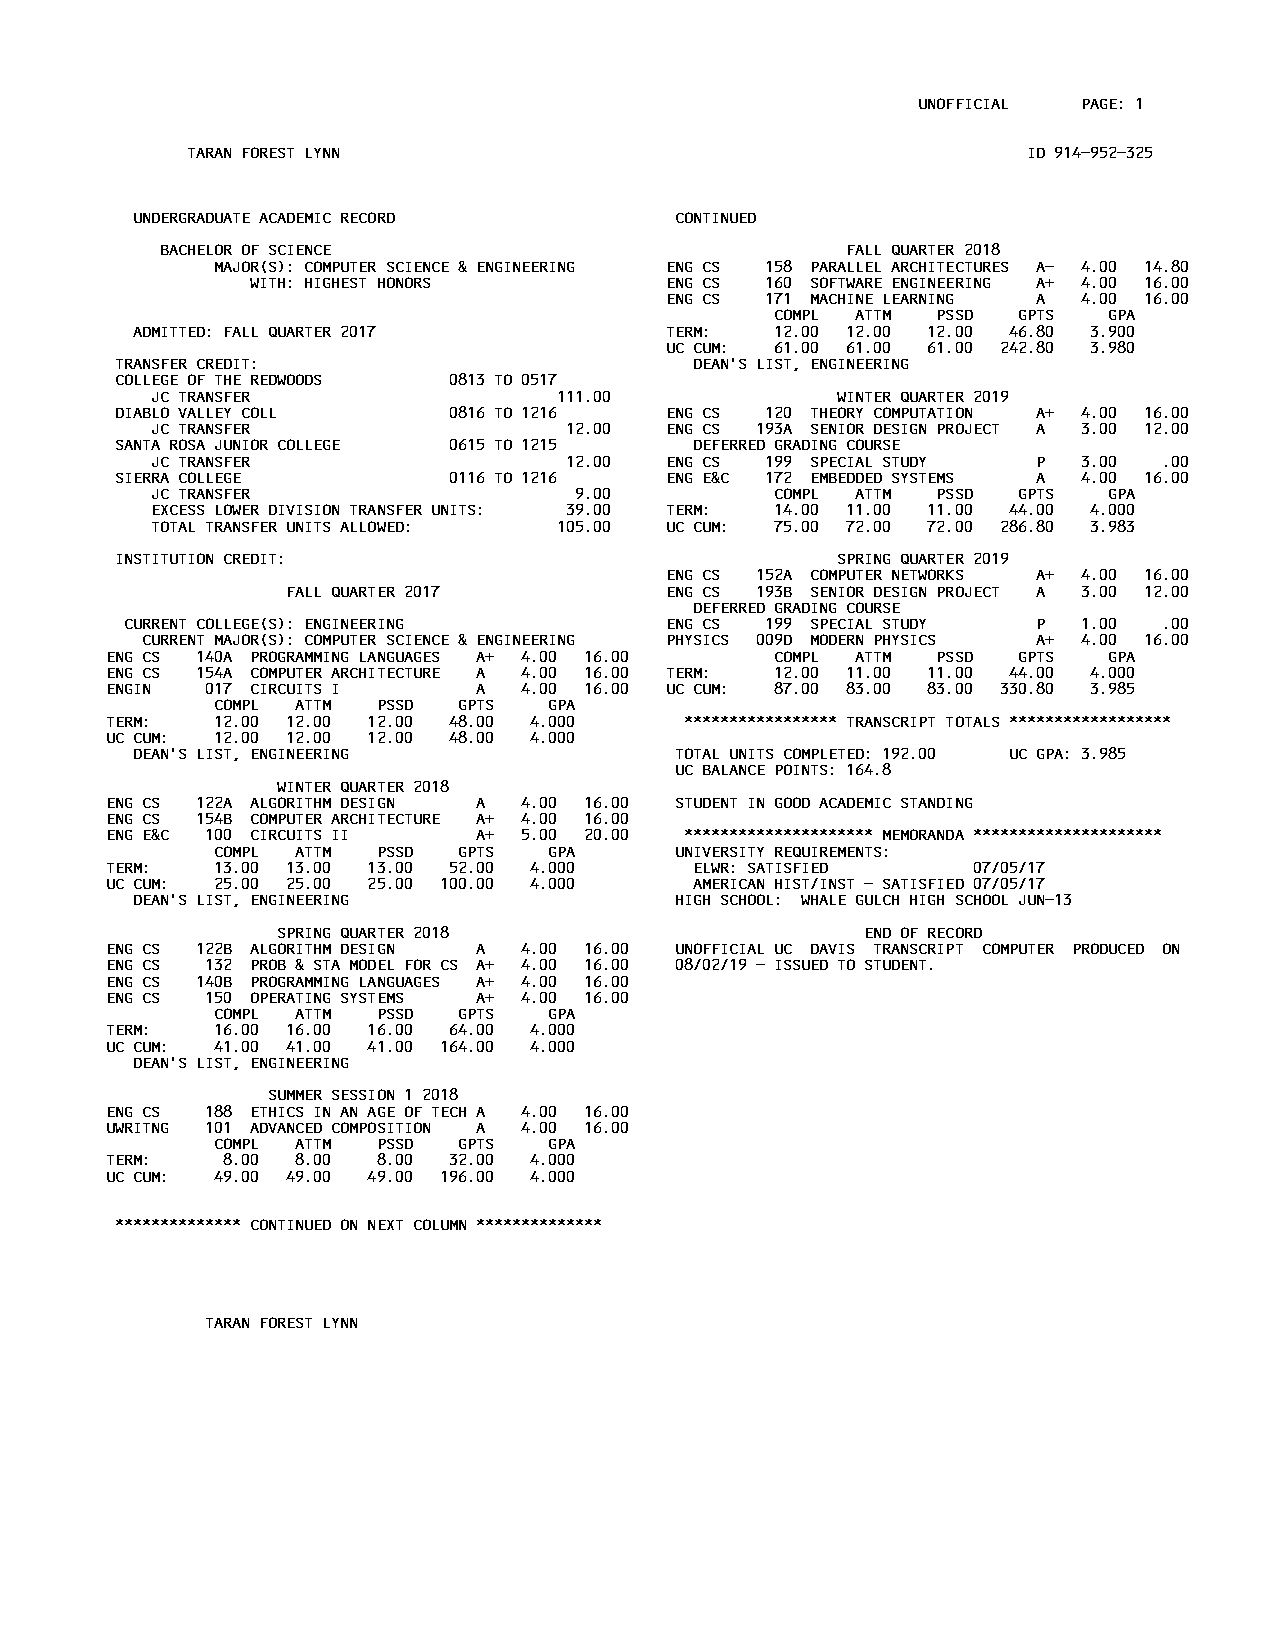
\includepdf{unofficial_trans.pdf}

\end{document}

